\documentclass{standalone}
\usepackage{tikz}
\usetikzlibrary{patterns, positioning}


\begin{document}
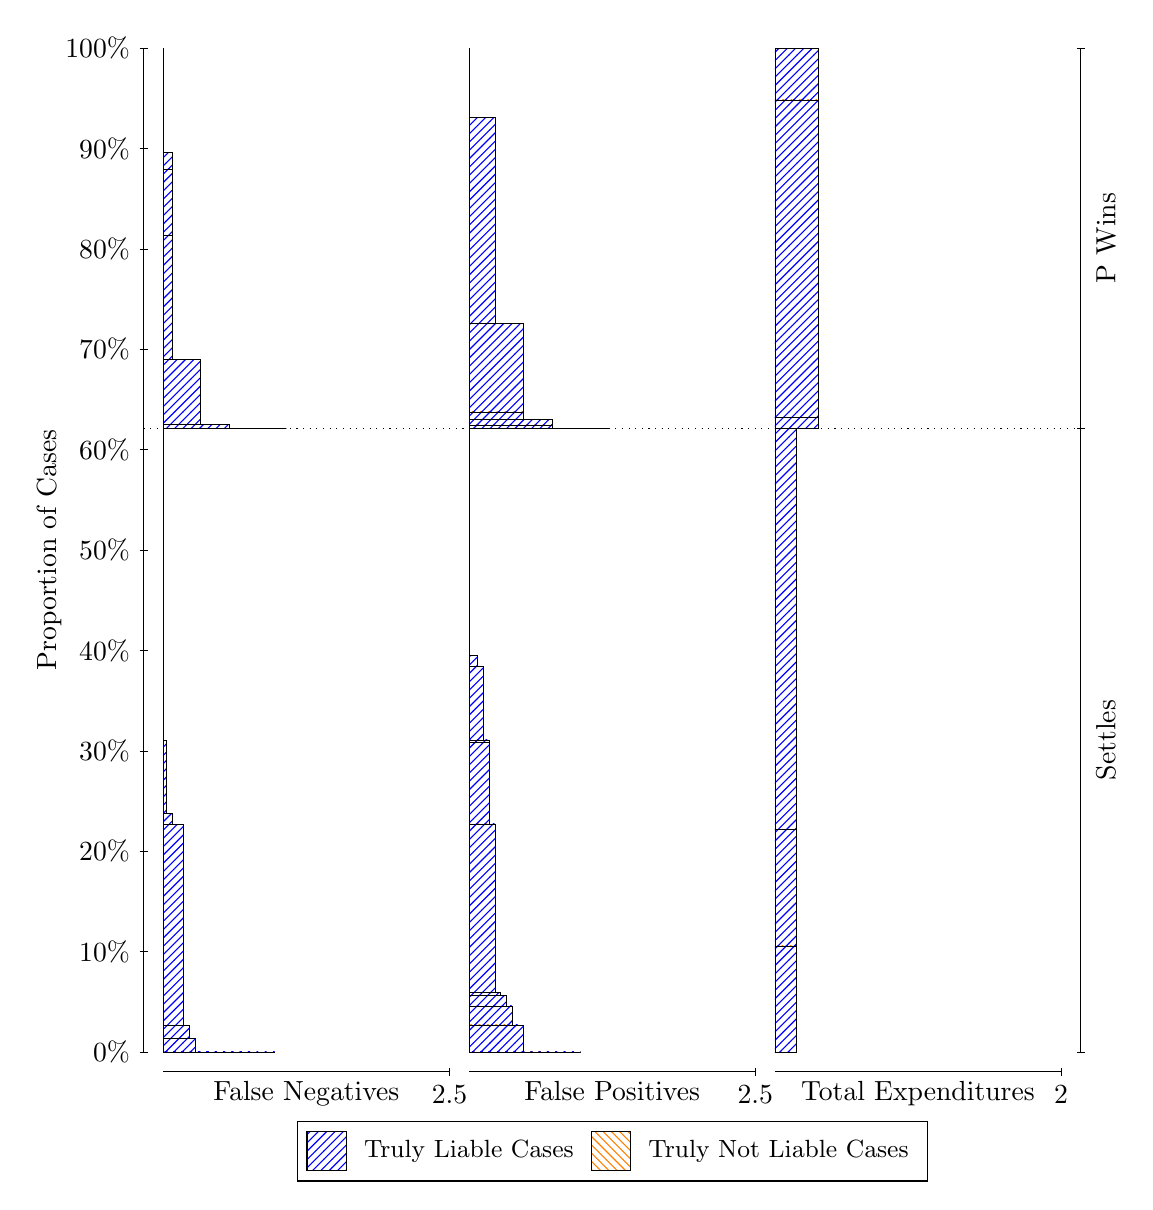
\begin{tikzpicture}
\draw[black, very thin] (1.5,1.75) -- (1.5,14.5);
\node[rotate=90, text=black, anchor=center] at (0.3, 8.125) {Proportion of Cases};
\draw[black, very thin] (1.45,1.75) -- (1.55,1.75);
\node[text=black, anchor=east] at (1.45, 1.75) {0\%};
\draw[black, very thin] (1.45,3.025) -- (1.55,3.025);
\node[text=black, anchor=east] at (1.45, 3.025) {10\%};
\draw[black, very thin] (1.45,4.3) -- (1.55,4.3);
\node[text=black, anchor=east] at (1.45, 4.3) {20\%};
\draw[black, very thin] (1.45,5.575) -- (1.55,5.575);
\node[text=black, anchor=east] at (1.45, 5.575) {30\%};
\draw[black, very thin] (1.45,6.85) -- (1.55,6.85);
\node[text=black, anchor=east] at (1.45, 6.85) {40\%};
\draw[black, very thin] (1.45,8.125) -- (1.55,8.125);
\node[text=black, anchor=east] at (1.45, 8.125) {50\%};
\draw[black, very thin] (1.45,9.4) -- (1.55,9.4);
\node[text=black, anchor=east] at (1.45, 9.4) {60\%};
\draw[black, very thin] (1.45,10.675) -- (1.55,10.675);
\node[text=black, anchor=east] at (1.45, 10.675) {70\%};
\draw[black, very thin] (1.45,11.95) -- (1.55,11.95);
\node[text=black, anchor=east] at (1.45, 11.95) {80\%};
\draw[black, very thin] (1.45,13.225) -- (1.55,13.225);
\node[text=black, anchor=east] at (1.45, 13.225) {90\%};
\draw[black, very thin] (1.45,14.5) -- (1.55,14.5);
\node[text=black, anchor=east] at (1.45, 14.5) {100\%};

\draw[black, very thin] (13.4,1.75) -- (13.4,14.5);
\draw[black, very thin] (13.35,1.75) -- (13.45,1.75);
\node[anchor=west] at (13.35, 1.75) {};
\draw[black, very thin] (13.35,9.6725) -- (13.45,9.6725);
\node[anchor=west] at (13.35, 9.6725) {};
\draw[black, very thin] (13.35,14.5) -- (13.45,14.5);
\node[anchor=west] at (13.35, 14.5) {};

\draw[black, very thin, pattern color=blue, pattern=north east lines] (1.75,1.75) rectangle (3.167,1.75);
\draw[black, very thin, pattern color=blue, pattern=north east lines] (1.75,1.75) rectangle (2.8763,1.75);
\draw[black, very thin, pattern color=blue, pattern=north east lines] (1.75,1.75) rectangle (2.8037,1.75);
\draw[black, very thin, pattern color=blue, pattern=north east lines] (1.75,1.75) rectangle (2.5857,1.75);
\draw[black, very thin, pattern color=blue, pattern=north east lines] (1.75,1.75) rectangle (2.513,1.7503);
\draw[black, very thin, pattern color=blue, pattern=north east lines] (1.75,1.7503) rectangle (2.4403,1.7505);
\draw[black, very thin, pattern color=blue, pattern=north east lines] (1.75,1.7505) rectangle (2.295,1.7505);
\draw[black, very thin, pattern color=blue, pattern=north east lines] (1.75,1.7505) rectangle (2.2223,1.7508);
\draw[black, very thin, pattern color=blue, pattern=north east lines] (1.75,1.7508) rectangle (2.1497,1.9219);
\draw[black, very thin, pattern color=blue, pattern=north east lines] (1.75,1.9219) rectangle (2.077,2.0923);
\draw[black, very thin, pattern color=blue, pattern=north east lines] (1.75,2.0923) rectangle (2.0043,4.6381);
\draw[black, very thin, pattern color=blue, pattern=north east lines] (1.75,4.6381) rectangle (1.9317,4.6396);
\draw[black, very thin, pattern color=blue, pattern=north east lines] (1.75,4.6396) rectangle (1.859,4.7768);
\draw[black, very thin, pattern color=blue, pattern=north east lines] (1.75,4.7768) rectangle (1.7863,5.7105);
\draw[black, very thin, pattern color=orange, pattern=north west lines] (1.75,5.7105) rectangle (1.75,5.7105);
\draw[black, very thin, pattern color=blue, pattern=north east lines] (1.75,5.7105) rectangle (1.75,9.6725);
\draw[black, very thin, pattern color=blue, pattern=north east lines] (1.75,9.6725) rectangle (3.3123,9.6725);
\draw[black, very thin, pattern color=blue, pattern=north east lines] (1.75,9.6725) rectangle (2.949,9.6727);
\draw[black, very thin, pattern color=blue, pattern=north east lines] (1.75,9.6727) rectangle (2.5857,9.7231);
\draw[black, very thin, pattern color=blue, pattern=north east lines] (1.75,9.7231) rectangle (2.2223,10.548);
\draw[black, very thin, pattern color=blue, pattern=north east lines] (1.75,10.548) rectangle (2.2223,10.549);
\draw[black, very thin, pattern color=blue, pattern=north east lines] (1.75,10.549) rectangle (1.859,12.121);
\draw[black, very thin, pattern color=blue, pattern=north east lines] (1.75,12.121) rectangle (1.859,12.966);
\draw[black, very thin, pattern color=blue, pattern=north east lines] (1.75,12.966) rectangle (1.859,13.173);
\draw[black, very thin, pattern color=orange, pattern=north west lines] (1.75,13.173) rectangle (1.75,13.173);
\draw[black, very thin, pattern color=blue, pattern=north east lines] (1.75,13.173) rectangle (1.75,14.5);
\draw[black, very thin, pattern color=orange, pattern=north west lines] (5.6333,1.75) rectangle (7.0503,1.75);
\draw[black, very thin, pattern color=blue, pattern=north east lines] (5.6333,1.75) rectangle (7.0503,1.75);
\draw[black, very thin, pattern color=orange, pattern=north west lines] (5.6333,1.75) rectangle (6.7597,1.75);
\draw[black, very thin, pattern color=blue, pattern=north east lines] (5.6333,1.75) rectangle (6.7597,1.75);
\draw[black, very thin, pattern color=blue, pattern=north east lines] (5.6333,1.75) rectangle (6.687,1.7505);
\draw[black, very thin, pattern color=orange, pattern=north west lines] (5.6333,1.7505) rectangle (6.6143,1.7505);
\draw[black, very thin, pattern color=blue, pattern=north east lines] (5.6333,1.7505) rectangle (6.6143,1.7505);
\draw[black, very thin, pattern color=orange, pattern=north west lines] (5.6333,1.7505) rectangle (6.469,1.7505);
\draw[black, very thin, pattern color=blue, pattern=north east lines] (5.6333,1.7505) rectangle (6.469,1.7509);
\draw[black, very thin, pattern color=blue, pattern=north east lines] (5.6333,1.7509) rectangle (6.3963,1.7521);
\draw[black, very thin, pattern color=blue, pattern=north east lines] (5.6333,1.7521) rectangle (6.3237,2.0925);
\draw[black, very thin, pattern color=blue, pattern=north east lines] (5.6333,2.0925) rectangle (6.251,2.0939);
\draw[black, very thin, pattern color=orange, pattern=north west lines] (5.6333,2.0939) rectangle (6.1783,2.0939);
\draw[black, very thin, pattern color=blue, pattern=north east lines] (5.6333,2.0939) rectangle (6.1783,2.3356);
\draw[black, very thin, pattern color=blue, pattern=north east lines] (5.6333,2.3356) rectangle (6.1057,2.4732);
\draw[black, very thin, pattern color=blue, pattern=north east lines] (5.6333,2.4732) rectangle (6.033,2.505);
\draw[black, very thin, pattern color=blue, pattern=north east lines] (5.6333,2.505) rectangle (5.9603,4.647);
\draw[black, very thin, pattern color=orange, pattern=north west lines] (5.6333,4.647) rectangle (5.8877,4.647);
\draw[black, very thin, pattern color=blue, pattern=north east lines] (5.6333,4.647) rectangle (5.8877,5.68);
\draw[black, very thin, pattern color=blue, pattern=north east lines] (5.6333,5.68) rectangle (5.8877,5.7121);
\draw[black, very thin, pattern color=blue, pattern=north east lines] (5.6333,5.7121) rectangle (5.815,6.6458);
\draw[black, very thin, pattern color=blue, pattern=north east lines] (5.6333,6.6458) rectangle (5.7423,6.783);
\draw[black, very thin, pattern color=blue, pattern=north east lines] (5.6333,6.783) rectangle (5.6697,6.7844);
\draw[black, very thin, pattern color=blue, pattern=north east lines] (5.6333,6.7844) rectangle (5.6333,9.6725);
\draw[black, very thin, pattern color=orange, pattern=north west lines] (5.6333,9.6725) rectangle (7.4137,9.6725);
\draw[black, very thin, pattern color=blue, pattern=north east lines] (5.6333,9.6725) rectangle (7.4137,9.6725);
\draw[black, very thin, pattern color=blue, pattern=north east lines] (5.6333,9.6725) rectangle (7.0503,9.6731);
\draw[black, very thin, pattern color=orange, pattern=north west lines] (5.6333,9.6731) rectangle (7.0503,9.6731);
\draw[black, very thin, pattern color=blue, pattern=north east lines] (5.6333,9.6731) rectangle (7.0503,9.6738);
\draw[black, very thin, pattern color=blue, pattern=north east lines] (5.6333,9.6738) rectangle (6.687,9.7149);
\draw[black, very thin, pattern color=orange, pattern=north west lines] (5.6333,9.7149) rectangle (6.687,9.7149);
\draw[black, very thin, pattern color=blue, pattern=north east lines] (5.6333,9.7149) rectangle (6.687,9.7828);
\draw[black, very thin, pattern color=blue, pattern=north east lines] (5.6333,9.7828) rectangle (6.3237,9.8779);
\draw[black, very thin, pattern color=orange, pattern=north west lines] (5.6333,9.8779) rectangle (6.3237,9.8779);
\draw[black, very thin, pattern color=blue, pattern=north east lines] (5.6333,9.8779) rectangle (6.3237,10.999);
\draw[black, very thin, pattern color=blue, pattern=north east lines] (5.6333,10.999) rectangle (5.9603,11.002);
\draw[black, very thin, pattern color=orange, pattern=north west lines] (5.6333,11.002) rectangle (5.9603,11.002);
\draw[black, very thin, pattern color=blue, pattern=north east lines] (5.6333,11.002) rectangle (5.9603,13.623);
\draw[black, very thin, pattern color=blue, pattern=north east lines] (5.6333,13.623) rectangle (5.6333,14.5);
\draw[black, very thin, pattern color=orange, pattern=north west lines] (9.5167,1.75) rectangle (9.7892,1.75);
\draw[black, very thin, pattern color=blue, pattern=north east lines] (9.5167,1.75) rectangle (9.7892,3.0968);
\draw[black, very thin, pattern color=orange, pattern=north west lines] (9.5167,3.0968) rectangle (9.7892,3.0968);
\draw[black, very thin, pattern color=blue, pattern=north east lines] (9.5167,3.0968) rectangle (9.7892,4.5743);
\draw[black, very thin, pattern color=orange, pattern=north west lines] (9.5167,4.5743) rectangle (9.7892,4.5743);
\draw[black, very thin, pattern color=blue, pattern=north east lines] (9.5167,4.5743) rectangle (9.7892,9.6725);
\draw[black, very thin, pattern color=orange, pattern=north west lines] (9.5167,9.6725) rectangle (10.062,9.6725);
\draw[black, very thin, pattern color=blue, pattern=north east lines] (9.5167,9.6725) rectangle (10.062,9.812);
\draw[black, very thin, pattern color=orange, pattern=north west lines] (9.5167,9.812) rectangle (10.062,9.812);
\draw[black, very thin, pattern color=blue, pattern=north east lines] (9.5167,9.812) rectangle (10.062,13.841);
\draw[black, very thin, pattern color=orange, pattern=north west lines] (9.5167,13.841) rectangle (10.062,13.841);
\draw[black, very thin, pattern color=blue, pattern=north east lines] (9.5167,13.841) rectangle (10.062,14.5);
\draw[black, dotted] (1.5,9.6725) -- (13.4,9.6725);
\draw[black, very thin] (1.75,1.5) -- (5.3833,1.5);
\node[text=black, anchor=north] at (3.5667, 1.5) {False Negatives};
\draw[black, very thin] (5.3833,1.45) -- (5.3833,1.55);
\node[text=black, anchor=north] at (5.3833, 1.45) {2.5};

\draw[black, very thin] (5.6333,1.5) -- (9.2667,1.5);
\node[text=black, anchor=north] at (7.45, 1.5) {False Positives};
\draw[black, very thin] (9.2667,1.45) -- (9.2667,1.55);
\node[text=black, anchor=north] at (9.2667, 1.45) {2.5};

\draw[black, very thin] (9.5167,1.5) -- (13.15,1.5);
\node[text=black, anchor=north] at (11.333, 1.5) {Total Expenditures};
\draw[black, very thin] (13.15,1.45) -- (13.15,1.55);
\node[text=black, anchor=north] at (13.15, 1.45) {2};

\node[text=black, centered, rotate=90] at (13.72, 5.7113) {Settles};
\node[text=black, centered, rotate=90] at (13.72, 12.086) {P Wins};

\draw (7.449999999999999,1.5) node[draw=none] (baseCoordinate) {};
\begin{scope}[align=center]
        \matrix[scale=0.5, draw=black, below=0.5cm of baseCoordinate, nodes={draw}, column sep=0.1cm]{
            \node[rectangle, draw, minimum width=0.5cm, minimum height=0.5cm, pattern color=blue, pattern=north east lines] {}; &
            \node[draw=none, font=\small, text=black] (B) {Truly Liable Cases}; &
            \node[rectangle, draw, minimum width=0.5cm, minimum height=0.5cm, pattern color=orange, pattern=north west lines] {}; &
            \node[draw=none, font=\small, text=black] (B) {Truly Not Liable Cases}; \\
            };
\end{scope}

\end{tikzpicture}
\end{document}